\documentclass[11pt,a4paper]{article}
\usepackage[utf8]{inputenc}
\setlength{\parindent}{0em}
\setlength{\parskip}{1.0em}

\usepackage{natbib}
\usepackage{geometry}

\usepackage{graphicx}
\graphicspath{ {./images/} }

\usepackage{tikz}
\usetikzlibrary{fit,positioning}

\usepackage{amsmath}
\usepackage{amsfonts}
\usepackage{amssymb}

%to do notes stuff 
\usepackage{todonotes}
\newcommand{\sttodo}[2][]
{\todo[caption={\textbf{TG}}, size=\small, color = orange, #1]{#2}~}
\newcommand{\ttodo}[2][]
{\vspace{0.1cm}\hfil \todo[caption={\textbf{TG}}, size=\small, color = orange, inline, #1]{#2}}

\begin{document}

% Title and author info
\title{Compositional Explanations: A Proposal}
\author{Joey Velez-Ginorio}
\maketitle

\clearpage 
\tableofcontents
\clearpage 



\section{Model}

Given an arbitrary physical simulation, and an event we care about, a model of explanations should compute a distribution over explanations of that event. Something like the following list, but with probabilities associated with each item.

\begin{itemize}
	\item \textit{(Event) because (Cause1)}
	\item \textit{(Event) because ((Cause1) or (Cause2))}
	\item \textit{(Event) because ((Cause1) and (Cause2))}
	\item \textit{(Event) because (((Cause1) and (Cause2)) or ((Cause3) and (Cause4)))}
	\item \textit{....}
\end{itemize}


In order to get that distribution, we frame the task as a problem of Bayesian inference. Formally, how do we compute:

\begin{equation}
P(\text{Explanation}|\text{World}, \text{Event})  
\end{equation}

If we specify a generative model, we can use it to guide how we compute this distribution. With it, we also have a convenient way to partition the mechanisms of our model, separating parts that compute different elements of the distribution. This will be discussed after introducing the generative model in figure \ref{fig:gen_model}.

\begin{figure}[ht]
	\centering
	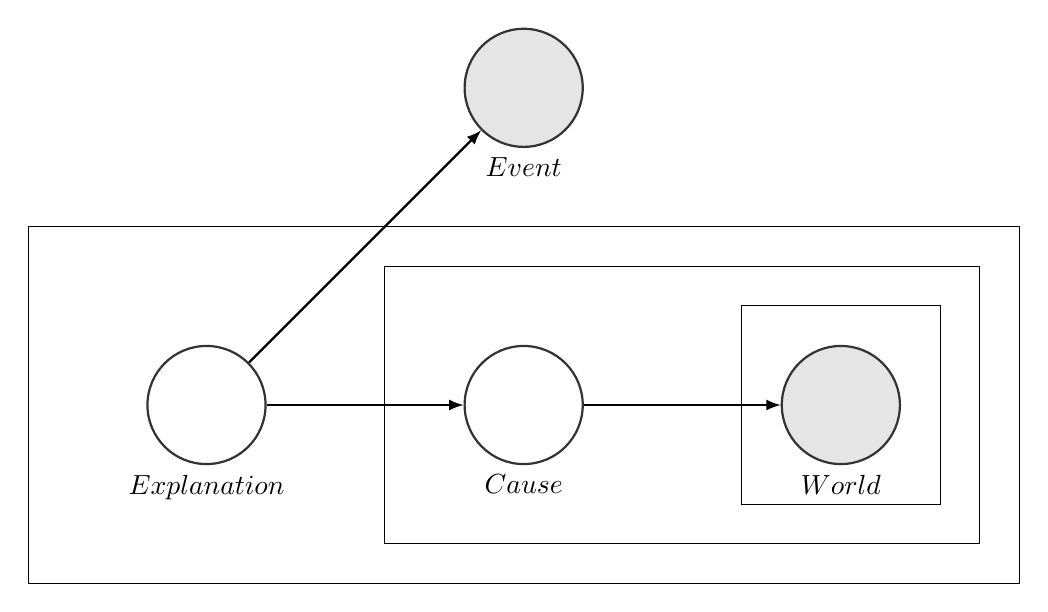
\begin{tikzpicture}
	\tikzstyle{main}=[circle, minimum size = 15mm, thick, draw =black!80, 							node distance = 25mm]
	\tikzstyle{connect}=[-latex, thick]
	\tikzstyle{box}=[rectangle, draw=black!100]
	  \node[main] (exp) [label=below:$Explanation$] { };
	  \node[main] (cau) [right=of exp,label=below:$Cause$] {};
	  \node[main, fill = black!10] (eve) [above=of cau,label=below:$Event				$] { };
	  \node[main, fill = black!10] (w) [right=of cau,label=below:$World$] 				{ };
	  \path (exp) edge [connect] (cau)
			(cau) edge [connect] (w)
			(exp) edge [connect] (eve);

	  \node[rectangle, inner sep=5mm, draw=black!100, fit = (w)] {};
	  \node[rectangle, inner sep=10mm,draw=black!100, fit= (cau) (w)] {};
	  \node[rectangle, inner sep=15mm, draw=black!100, fit = (exp) (cau) 				(w)] {};

	\end{tikzpicture}
	
	\caption{Our generative model}
	\label{fig:gen_model}
\end{figure}

You can view each node in the generative model as a random variable, and each edge as encoding the statistical dependencies of those random variables. We should be able to infer information about upstream nodes from observations of downstream nodes. Knowledge of the world lets us infer cause, knowledge of cause and the event of interest allow us to infer explanation. The boxes are meant to highlight that the generative model is composed of smaller models. At the core, is a model of the world provided by a physics engine, succeeded by a counterfactual-based model of cause, and lastly the model of explanation we pursue in this proposal.

The relationship between these random variables are captured nicely by using the generative model to derive a joint distribution. Note, from here on out, I will use abbreviated notation for the random variables: $Ex$ for $Explanation$, $C$ for $Cause$, $Ev$ for $Event$, and $W$ for $World$.

\begin{equation}
P(Ex, C, Ev, W) = \\ P(W|C)P(C|Ex)P(Ev|Ex)P(Ex)
\end{equation}

\subsection{Posterior}

With the joint distribution, we can return to our definition of equation 1, and define a posterior distribution over explanations:

\begin{equation}
\begin{split}
P(Ex|W,Ev) & \propto P(W,Ev|Ex)P(Ex)\\ 
		& \propto P(W|Ex)P(Ev|Ex)P(Ex)\\
		& \propto \sum_{C} (P(W|C)P(C|Ex))P(Ev|Ex)P(Ex)
\end{split}
\end{equation}

%To make the expansion clear, we first use bayes rule to set $P(Ex|W,Ev)$ proportional to the likelihood, $P(W,Ev|Ex)$, and the prior, $P(Ex)$. Then, because of the conditional independence of $W$ and $Ev$ given $Ex$, we can express the likelihood as $P(W|Ex)P(Ev|Ex)$. Lastly, we marginalize over $C$ to express $P(W|Ex)$ as $\sum_{C} (P(W|C)P(C|E))$. In final form, the bayes formulation is in terms of distributions provided by the joint distribution specified earlier, which with the generative model we should be able to compute.

Our definition of the posterior definition helps us capture two intuitions about explanations. The likelihood, $P(W,Ev|Ex)$, should favor explanations that invoke relevant causes and that mention the event we're interested in. The prior, $P(Ex)$,  should favor simple over complex explanations. In the following sections we discuss what it means to invoke a relevant cause, and what it means for an explanation to be simple or complex -- and how to include these intuitions in our computation.

\subsection{Likelihood, $P(W,Ev|Ex)$}

The likelihood should favor explanations that invoke relevant causes from what happened in the world, and that include the event we're interested in explaining. The expansion of the likelihood helps us achieve this. We will discuss each of the terms in more detail.

\begin{equation}
P(W,Ev|Ex) = P(W|Ex)P(Ev|Ex)
\end{equation}

\subsubsection{$P(Ev|Ex)$}

The chance that an event occurred given an explanation can be treated as binary choice. It's 1 if the event was mentioned in the explanation and 0 if the event was not mentioned in the explanation.

\ttodo{This assumption is interesting but might be too strong -- }


\subsubsection{$P(W|Ex)$}

The chance that you saw what happened in the world because of causes invoked in an explanation would be high if the causes mattered. However, $P(W|Ex)$ does not express this intuition until we marginalize over all invoked causes in the explanation. 

\begin{equation}
P(W|Ex) = \sum_{C} P(W|C)P(C|Ex)
\end{equation}


Drawing on the approach of Gerstenberg et al. \citep{gerstenberg2015whether}, we say that the probability of the world given a cause, $P(W|C)$, is high when the cause invoked is a \textit{difference maker}. Otherwise, if the cause invoked would have made no or little difference to the observed world, it's value should be representative of the degree of influence. See \citep{gerstenberg2015whether} for specific details on what constitutes a cause as a \textit{difference maker}. $P(C|Ex)$, can be treated as uniform for all causes, this term captures the assumption that all causes invoked in an explanation are equally important (not always true but reasonable in our task setting).

\subsection{Prior, $P(Ex)$}
The prior should favor explanations that are simple. To accomplish this we can set the prior to be negative exponential in the number of causes invoked in the explanation, $x$. 

\begin{equation}
P(Ex) = e^{-x} 
\end{equation}

\bibliographystyle{abbrv}
\bibliography{proposal}

\end{document}